\documentclass[11pt,a4paper]{article}
\usepackage[utf8]{vietnam}
\usepackage{amsmath,amssymb}
\usepackage{geometry}
\geometry{top=1.5cm,bottom=1.2cm,left=1.4cm,right=1.4cm,headheight=28pt,headsep=12pt,footskip=18pt}
\usepackage{tikz}
\usepackage{xcolor}
\usepackage{graphicx}
\usepackage{fancyhdr}
\usepackage{tabularx}
\usepackage{enumitem}

\renewcommand{\baselinestretch}{1.08}
\setlength{\parskip}{2pt}
\setlength{\parindent}{0pt}

\definecolor{hfRed}{RGB}{211,47,47}
\definecolor{hfGreen}{RGB}{139,195,144}
\definecolor{myGreen}{RGB}{46,125,50}
\definecolor{myBlue}{RGB}{21,101,192}
\definecolor{mySub}{RGB}{0,105,92}
\definecolor{myPurple}{RGB}{106,27,154}

\pagestyle{fancy}
\fancyhf{}
\fancyhead[L]{\small\itshape\color{hfRed} Tài liệu lưu hành nội bộ}
\fancyhead[R]{\small\itshape\color{hfRed} Thầy \textbf{TRẦN VĂN THẠNH} - 0777.470.803}
\renewcommand{\headrulewidth}{0.8pt}
\renewcommand{\headrule}{\hbox to\headwidth{\color{hfGreen}\leaders\hrule height \headrulewidth\hfill}}

\fancyfoot[L]{\small\itshape\color{hfRed} CS1: 6/15 Nguyễn Hoàng, P. Kim Long, TP Huế \quad|\quad CS2: 24 Đặng Thái Thân, TP Huế}
\fancyfoot[R]{\small\bfseries\color{hfRed} Trang \thepage}
\renewcommand{\footrulewidth}{0.8pt}
\renewcommand{\footrule}{\hbox to\headwidth{\color{hfGreen}\leaders\hrule height \footrulewidth\hfill}}

\begin{document}

% --- HEADER BLOCK ---
\begin{tabularx}{\textwidth}{@{}l X r@{}}
\textbf{\small SỞ GIÁO DỤC VÀ ĐÀO TẠO} & & \textbf{\small ĐỀ KIỂM TRA GIỮA HỌC KÌ I} \\
\textbf{\normalsize TRƯỜNG THPT CHUYÊN / THPT} & & \textbf{\normalsize MÔN: HÓA HỌC - LỚP 10} \\
\textit{\small (Đề thi gồm có 03 trang)} & & \textit{\small Thời gian làm bài: 45 phút (không kể phát đề)}
\end{tabularx}

\begin{center}
{\color{red!80!black}\textbf{(BẢN GIÁO VIÊN -- CÓ ĐÁP ÁN \& LỜI GIẢI CHI TIẾT)}}\par\vspace{3pt}
\textbf{Họ và tên thí sinh:} \dotfill \quad \textbf{Lớp:} \dots\dots\dots \quad \textbf{Số báo danh:} \dots\dots\dots \hfill \textbf{\large Mã đề 101}
\end{center}
\vspace{-4pt}
{\color{gray!50}\hrule height 0.8pt}
\vspace{6pt}

% =============================================================================
% PHẦN I
% =============================================================================
{\color{myGreen}\bfseries\large PHẦN I (3,0 ĐIỂM). Câu trắc nghiệm nhiều phương án lựa chọn.}

\textit{\small Thí sinh trả lời từ câu 1 đến câu 12. Mỗi câu hỏi thí sinh chỉ chọn một phương án.}
\vspace{3pt}

% CÂU 1
\textbf{Câu 1.} Phát biểu nào sau đây \textbf{không đúng}?
\begin{enumerate}[label=\textbf{\Alph*.},leftmargin=*,itemsep=1pt,topsep=1pt]
\item Số khối của hạt nhân bằng tổng số proton và số neutron.
\item Nguyên tố hoá học là những nguyên tử có cùng số đơn vị điện tích hạt nhân.
\item Số hiệu nguyên tử bằng số đơn vị điện tích hạt nhân nguyên tử.
\item \textbf{\color{red} Trong nguyên tử, số đơn vị điện tích hạt nhân bằng số proton và bằng số neutron.}
\end{enumerate}
\begin{quote}\small
{\color{myBlue}\textbf{$\triangleright$ Lời giải chi tiết:}} Đáp án đúng: \textbf{\color{red} D}\\
Trong nguyên tử trung hòa về điện, số đơn vị điện tích hạt nhân bằng số proton và bằng số electron ($Z = p = e$). Số neutron ($N$) trong hạt nhân không nhất thiết phải bằng số proton (trừ một số ít nguyên tử nhẹ như $^4_2\text{He}, ^{12}_6\text{C}, ^{14}_7\text{N}, ^{16}_8\text{O}$). Do đó phát biểu D là không đúng.
\end{quote}
\vspace{2pt}


% CÂU 2
\textbf{Câu 2.} Nguyên tử chứa những hạt mang điện là
\begin{enumerate}[label=\textbf{\Alph*.},leftmargin=*,itemsep=1pt,topsep=1pt]
\item \textbf{\color{red} proton và electron.}
\item proton và $\alpha$.
\item electron và neutron.
\item proton và neutron.
\end{enumerate}
\begin{quote}\small
{\color{myBlue}\textbf{$\triangleright$ Lời giải chi tiết:}} Đáp án đúng: \textbf{\color{red} A}\\
Nguyên tử được cấu tạo từ ba loại hạt cơ bản: proton (mang điện tích dương $+1$), electron (mang điện tích âm $-1$), và neutron (không mang điện). Do đó, các hạt mang điện trong nguyên tử gồm proton và electron.
\end{quote}
\vspace{2pt}


% CÂU 3
\textbf{Câu 3.} Sự phân bố electron theo orbital nào dưới đây là đúng?
\begin{center}
\begin{tabularx}{\textwidth}{*{4}{>{\centering\arraybackslash}X}}
\textbf{A.} \raisebox{-0.3\height}{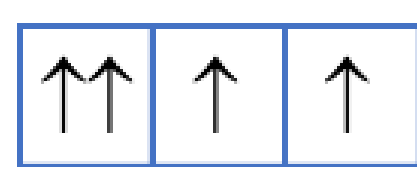
\includegraphics[height=0.9cm]{images_hoa10/page_1_img_1_48.png}} & 
\textbf{\color{red} B.} \raisebox{-0.3\height}{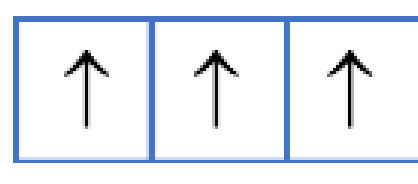
\includegraphics[height=0.9cm]{images_hoa10/page_1_img_2_50.png}} & 
\textbf{C.} \raisebox{-0.3\height}{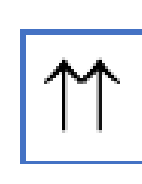
\includegraphics[height=0.9cm]{images_hoa10/page_1_img_3_52.png}} & 
\textbf{D.} \raisebox{-0.3\height}{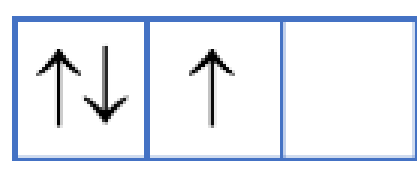
\includegraphics[height=0.9cm]{images_hoa10/page_1_img_4_54.png}} \\
\end{tabularx}
\end{center}
\begin{quote}\small
{\color{myBlue}\textbf{$\triangleright$ Lời giải chi tiết:}} Đáp án đúng: \textbf{\color{red} B}\\
- Phương án A: Ô orbital thứ nhất có 2 electron cùng chiều spin (cùng hướng lên $\uparrow\uparrow$), vi phạm nguyên lí Pauli.\\
- Phương án B: Cả 3 electron phân bố vào 3 orbital riêng biệt với chiều spin cùng hướng lên ($\uparrow$), thỏa mãn nguyên lí Pauli và quy tắc Hund.\\
- Phương án C: Một orbital có 2 electron cùng chiều spin $\uparrow\uparrow$, vi phạm nguyên lí Pauli.\\
- Phương án D: Có 3 electron nhưng 2 electron đã ghép đôi trong 1 orbital trong khi còn 1 orbital trống, vi phạm quy tắc Hund.
\end{quote}
\vspace{2pt}


% CÂU 4
\textbf{Câu 4.} Lớp L có số phân lớp electron bằng
\begin{tabularx}{\textwidth}{@{}XXXX@{}}
\textbf{A.} 1. & \textbf{B.} 4. & \textbf{\color{red} C. 2.} & \textbf{D.} 3. \\
\end{tabularx}
\begin{quote}\small
{\color{myBlue}\textbf{$\triangleright$ Lời giải chi tiết:}} Đáp án đúng: \textbf{\color{red} C}\\
Lớp L ứng với $n = 2$, có 2 phân lớp electron là phân lớp 2s và phân lớp 2p.
\end{quote}
\vspace{2pt}


% CÂU 5
\textbf{Câu 5.} Các hạt cấu tạo nên hạt nhân của hầu hết các nguyên tử là
\begin{tabularx}{\textwidth}{@{}XX@{}}
\textbf{A.} electron và neutron. & \textbf{B.} electron, proton và neutron. \\
\textbf{\color{red} C. proton và neutron.} & \textbf{D.} neutron và electron. \\
\end{tabularx}
\begin{quote}\small
{\color{myBlue}\textbf{$\triangleright$ Lời giải chi tiết:}} Đáp án đúng: \textbf{\color{red} C}\\
Hạt nhân của hầu hết các nguyên tử được cấu tạo từ hai loại hạt là proton và neutron (riêng nguyên tử hydrogen $^1_1\text{H}$ chỉ có 1 proton, không có neutron).
\end{quote}
\vspace{2pt}


% CÂU 6
\textbf{Câu 6.} Kí hiệu chung của mọi nguyên tử là $^{A}_{Z}\text{X}$, trong đó $A$, $Z$ và $\text{X}$ lần lượt là
\begin{enumerate}[label=\textbf{\Alph*.},leftmargin=*,itemsep=1pt,topsep=1pt]
\item \textbf{\color{red} số khối, số hiệu nguyên tử, kí hiệu nguyên tố.}
\item số khối, kí hiệu nguyên tố, số hiệu nguyên tử.
\item số hiệu nguyên tử, kí hiệu nguyên tố, số khối.
\item số hiệu nguyên tử, số khối, kí hiệu nguyên tố.
\end{enumerate}
\begin{quote}\small
{\color{myBlue}\textbf{$\triangleright$ Lời giải chi tiết:}} Đáp án đúng: \textbf{\color{red} A}\\
Theo quy ước quốc tế về kí hiệu nguyên tử $^{A}_{Z}\text{X}$: $A$ là số khối ($A = Z + N$), $Z$ là số hiệu nguyên tử, $\text{X}$ là kí hiệu nguyên tố hoá học.
\end{quote}
\vspace{2pt}


% CÂU 7
\textbf{Câu 7.} Nguyên tử của nguyên tố X có electron cuối cùng điền vào phân lớp $3p^1$. Nguyên tử của nguyên tố Y có electron cuối cùng điền vào phân lớp $3p^3$. Số proton của X, Y lần lượt là
\begin{tabularx}{\textwidth}{@{}XXXX@{}}
\textbf{A.} 12 và 14. & \textbf{\color{red} B. 13 và 15.} & \textbf{C.} 12 và 15. & \textbf{D.} 13 và 14. \\
\end{tabularx}
\begin{quote}\small
{\color{myBlue}\textbf{$\triangleright$ Lời giải chi tiết:}} Đáp án đúng: \textbf{\color{red} B}\\
- Cấu hình electron của X: $1s^2 2s^2 2p^6 3s^2 3p^1 \Rightarrow Z_\text{X} = 13$ (Aluminium - Al).\\
- Cấu hình electron của Y: $1s^2 2s^2 2p^6 3s^2 3p^3 \Rightarrow Z_\text{Y} = 15$ (Phosphorus - P).
\end{quote}
\vspace{2pt}


% CÂU 8
\textbf{Câu 8.} Orbital s có dạng
\begin{tabularx}{\textwidth}{@{}XXXX@{}}
\textbf{\color{red} A. hình cầu.} & \textbf{B.} hình số 8 nổi. & \textbf{C.} hình tròn. & \textbf{D.} hình bầu dục. \\
\end{tabularx}
\begin{quote}\small
{\color{myBlue}\textbf{$\triangleright$ Lời giải chi tiết:}} Đáp án đúng: \textbf{\color{red} A}\\
Orbital s có dạng hình cầu trong không gian 3 chiều; orbital p có dạng hình số 8 nổi gồm hai phần đối xứng qua hạt nhân.
\end{quote}
\vspace{2pt}


% CÂU 9
\textbf{Câu 9.} Dãy nào sau đây gồm các đồng vị của cùng một nguyên tố hoá học?
\begin{enumerate}[label=\textbf{\Alph*.},leftmargin=*,itemsep=1pt,topsep=1pt]
\item $^{14}_6\text{X}$, $^{14}_7\text{Y}$, $^{14}_8\text{Z}$.
\item \textbf{\color{red} $^{28}_{14}\text{X}$, $^{29}_{14}\text{Y}$, $^{30}_{14}\text{Z}$.}
\item $^{40}_{18}\text{X}$, $^{40}_{19}\text{Y}$, $^{40}_{20}\text{Z}$.
\item $^{19}_9\text{X}$, $^{19}_{10}\text{Y}$, $^{20}_{10}\text{Z}$.
\end{enumerate}
\begin{quote}\small
{\color{myBlue}\textbf{$\triangleright$ Lời giải chi tiết:}} Đáp án đúng: \textbf{\color{red} B}\\
Đồng vị là các nguyên tử có cùng số proton ($Z = 14$) nhưng khác nhau về số neutron dẫn đến số khối khác nhau ($A = 28, 29, 30$).
\end{quote}
\vspace{2pt}


% CÂU 10
\textbf{Câu 10.} Lithium ($Z = 3$) là một nguyên tố có nhiều công dụng, được sử dụng trong chế tạo máy bay và trong một số loại pin nhất định. Pin Lithium-Ion (Li-Ion) đang ngày càng phổ biến, nó cung cấp năng lượng cho cuộc sống của hàng triệu người mỗi ngày thông qua các thiết bị như máy tính xách tay, điện thoại di động, xe Hybrid, xe điện,… nhờ trọng lượng nhẹ, cung cấp năng lượng cao và khả năng sạc lại. Tính chất hóa học cơ bản của lithium là
\begin{tabularx}{\textwidth}{@{}XX@{}}
\textbf{A.} khí hiếm. & \textbf{B.} vừa kim loại vừa phi kim. \\
\textbf{\color{red} C. kim loại.} & \textbf{D.} phi kim. \\
\end{tabularx}
\begin{quote}\small
{\color{myBlue}\textbf{$\triangleright$ Lời giải chi tiết:}} Đáp án đúng: \textbf{\color{red} C}\\
Lithium ($Z = 3$) có cấu hình electron $1s^2 2s^1$, có 1 electron ở lớp ngoài cùng, thuộc nhóm IA nên là một kim loại kiềm điển hình.
\end{quote}
\vspace{2pt}


% CÂU 11
\textbf{Câu 11.} Cấu hình electron của nguyên tử P ($Z = 15$) là
\begin{tabularx}{\textwidth}{@{}XX@{}}
\textbf{A.} $1s^2 2s^2 2p^6 3s^2 3p^5$. & \textbf{\color{red} B. $1s^2 2s^2 2p^6 3s^2 3p^3$.} \\
\textbf{C.} $1s^2 2s^2 2p^6 3s^1$. & \textbf{D.} $1s^2 2s^2 2p^6 3s^2 3p^2$. \\
\end{tabularx}
\begin{quote}\small
{\color{myBlue}\textbf{$\triangleright$ Lời giải chi tiết:}} Đáp án đúng: \textbf{\color{red} B}\\
Nguyên tử P có $Z = 15$, electron điền theo mức năng lượng tăng dần: $1s^2 2s^2 2p^6 3s^2 3p^3$.
\end{quote}
\vspace{2pt}


% CÂU 12
\textbf{Câu 12.} Số proton và số neutron có trong một nguyên tử aluminium ($^{27}_{13}\text{Al}$) lần lượt là
\begin{tabularx}{\textwidth}{@{}XXXX@{}}
\textbf{A.} 12 và 14. & \textbf{\color{red} B. 13 và 14.} & \textbf{C.} 13 và 13. & \textbf{D.} 13 và 15. \\
\end{tabularx}
\begin{quote}\small
{\color{myBlue}\textbf{$\triangleright$ Lời giải chi tiết:}} Đáp án đúng: \textbf{\color{red} B}\\
Trong $^{27}_{13}\text{Al}$: Số proton $p = Z = 13$; số neutron $n = A - Z = 27 - 13 = 14$.
\end{quote}
\vspace{2pt}


% =============================================================================
% PHẦN II
% =============================================================================
\vspace{6pt}
{\color{myGreen}\bfseries\large PHẦN II (2,0 ĐIỂM). Câu trắc nghiệm đúng sai.}

\textit{\small Thí sinh trả lời từ câu 1 đến câu 2. Trong mỗi ý a), b), c), d) ở mỗi câu, thí sinh chọn đúng hoặc sai.}
\vspace{3pt}

% CÂU 1 PHẦN II
\textbf{Câu 1.} Cho hình ảnh một số nguyên tố sau trong bảng tuần hoàn:
\begin{center}
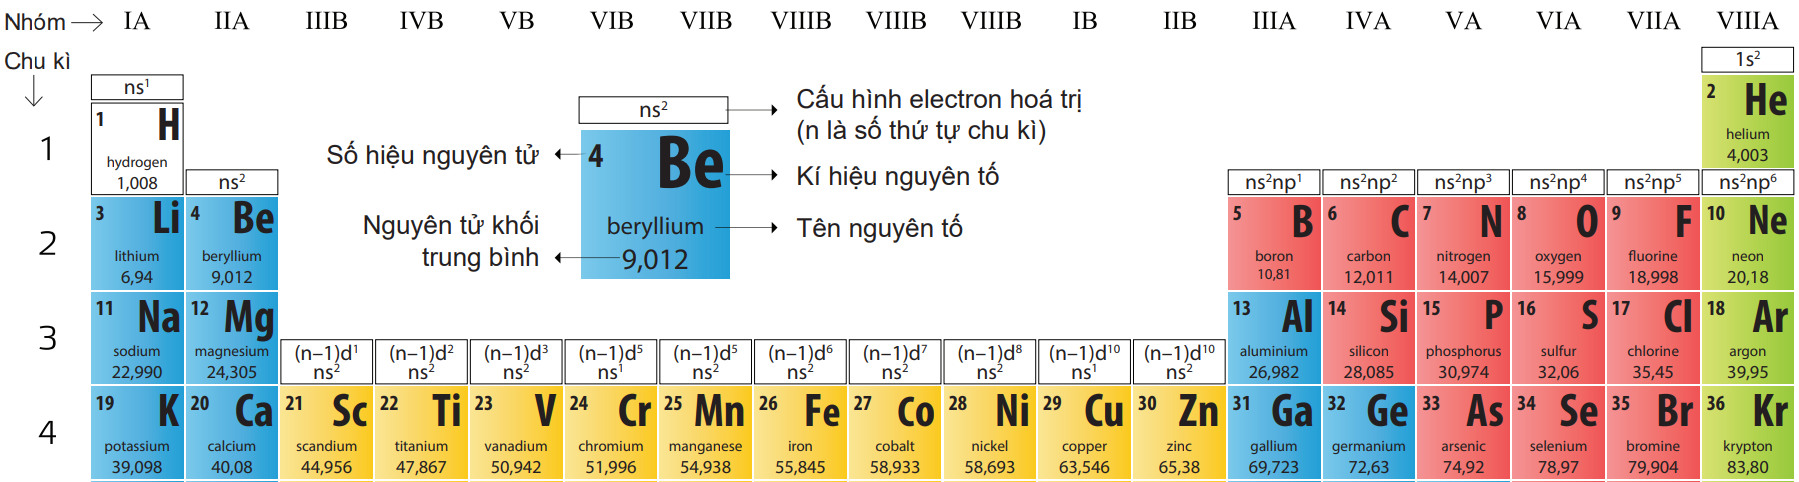
\includegraphics[width=0.98\textwidth]{images_hoa10/page_2_img_1_62.png}
\end{center}

\textit{Chọn đúng hoặc sai cho các kết luận sau:}\\
\textbf{a)} [\textbf{\color{red} ĐÚNG}] N và P có cùng số electron lớp ngoài cùng.\\
\begin{quote}\small
{\color{myBlue}\textbf{$\triangleright$ Giải thích ý a):}} N ($Z = 7$: $1s^2 2s^2 2p^3$) và P ($Z = 15$: $1s^2 2s^2 2p^6 3s^2 3p^3$) đều cùng thuộc nhóm VA nên đều có 5 electron ở lớp ngoài cùng ($ns^2 np^3$).
\end{quote}

\textbf{b)} [\textbf{\color{mySub} SAI}] Điện tích hạt nhân của S là $+32,06$.\\
\begin{quote}\small
{\color{myBlue}\textbf{$\triangleright$ Giải thích ý b):}} Giá trị 32,06 là nguyên tử khối trung bình của Sulfur. Sulfur có $Z = 16$ nên điện tích hạt nhân là $+16$.
\end{quote}

\textbf{c)} [\textbf{\color{red} ĐÚNG}] C và Li có cùng số lớp electron.\\
\begin{quote}\small
{\color{myBlue}\textbf{$\triangleright$ Giải thích ý c):}} C ($Z = 6$) và Li ($Z = 3$) đều thuộc chu kì 2 nên đều có 2 lớp electron.
\end{quote}

\textbf{d)} [\textbf{\color{red} ĐÚNG}] Có tổng 18 nguyên tố hóa học ở các chu kì nhỏ.\\
\begin{quote}\small
{\color{myBlue}\textbf{$\triangleright$ Giải thích ý d):}} Các chu kì nhỏ gồm: Chu kì 1 (2 nguyên tố), Chu kì 2 (8 nguyên tố), Chu kì 3 (8 nguyên tố). Tổng số nguyên tố là $2 + 8 + 8 = 18$.
\end{quote}


% CÂU 2 PHẦN II
\textbf{Câu 2.} Năm 1911, Rơ-đơ-pho (E. Rutherford) và các cộng sự đã dùng các hạt $\alpha$ bắn phá lá vàng mỏng và dùng màn huỳnh quang đặt sau lá vàng để theo dõi đường đi của các hạt $\alpha$. Đa số hạt $\alpha$ xuyên qua nguyên tử, một số hạt va chạm hạt nhân nguyên tử bị bật ngược trở lại hoặc bật ra hướng khác. Kết quả thí nghiệm đã rút ra các kết luận về nguyên tử như sau:

\textit{Chọn đúng hoặc sai cho các kết luận sau:}\\
\textbf{a)} [\textbf{\color{mySub} SAI}] Nguyên tử rỗng là nguyên nhân vì sao thể tích chất khí giảm một nửa khi tăng gấp đôi áp suất trong cùng điều kiện nhiệt độ.\\
\begin{quote}\small
{\color{myBlue}\textbf{$\triangleright$ Giải thích ý a):}} Thể tích chất khí giảm khi tăng áp suất là do khoảng cách giữa các phân tử khí rất lớn, không phải do cấu tạo rỗng bên trong bản thân mỗi nguyên tử.
\end{quote}

\textbf{b)} [\textbf{\color{red} ĐÚNG}] Hạt nhân nguyên tử có kích thước rất nhỏ so với kích thước nguyên tử.\\
\begin{quote}\small
{\color{myBlue}\textbf{$\triangleright$ Giải thích ý b):}} Hầu hết các hạt $\alpha$ đi thẳng qua lá vàng mà không bị lệch hướng chứng minh hạt nhân mang điện dương có kích thước vô cùng nhỏ bé so với kích thước nguyên tử.
\end{quote}

\textbf{c)} [\textbf{\color{red} ĐÚNG}] Hạt nhân nguyên tử tương đối đặc khít nên có một số hạt $\alpha$ bị bật ngược trở lại.\\
\begin{quote}\small
{\color{myBlue}\textbf{$\triangleright$ Giải thích ý c):}} Hạt nhân tập trung hầu như toàn bộ khối lượng nguyên tử nên có mật độ vật chất rất lớn (đặc khít). Khi hạt $\alpha$ va chạm trực diện với hạt nhân vàng thì bị bật ngược trở lại.
\end{quote}

\textbf{d)} [\textbf{\color{red} ĐÚNG}] Nguyên tử có cấu tạo rỗng nên hạt $\alpha$ xuyên qua được.\\
\begin{quote}\small
{\color{myBlue}\textbf{$\triangleright$ Giải thích ý d):}} Đại đa số hạt $\alpha$ đi thẳng qua lá vàng chứng minh phần lớn không gian trong nguyên tử là rỗng.
\end{quote}


% =============================================================================
% PHẦN III
% =============================================================================
\vspace{6pt}
{\color{myGreen}\bfseries\large PHẦN III (2,0 ĐIỂM). Câu trắc nghiệm trả lời ngắn.}

\textit{\small Thí sinh trả lời từ câu 1 đến câu 8.}
\vspace{3pt}

\textbf{Câu 1.} Kẽm là kim loại có ứng dụng quan trọng để bảo vệ sắt. Kí hiệu nguyên tử là $^{65}_{30}\text{Zn}$. Tính tổng số hạt proton, neutron và electron trong nguyên tử Zn.\\
\begin{quote}\small
{\color{myBlue}\textbf{$\triangleright$ Đáp án:}} \textbf{\color{red} 95}\\
Trong nguyên tử $^{65}_{30}\text{Zn}$: $p = e = 30$, $n = 65 - 30 = 35$. Tổng số hạt $= 30 + 35 + 30 = 95$.
\end{quote}


\textbf{Câu 2.} Potassium (K) là kim loại có tính khử mạnh, phân mức năng lượng cao nhất là $4s^1$. Tổng số electron lớp thứ 3 của K bằng bao nhiêu?\\
\begin{quote}\small
{\color{myBlue}\textbf{$\triangleright$ Đáp án:}} \textbf{\color{red} 8}\\
Cấu hình electron nguyên tử K ($Z = 19$): $1s^2 2s^2 2p^6 3s^2 3p^6 4s^1$. Lớp thứ 3 gồm phân lớp $3s$ và $3p$, có tổng số electron là $2 + 6 = 8$.
\end{quote}


\textbf{Câu 3.} Nguyên tố X thuộc chu kì 2. Vậy X có bao nhiêu lớp electron?\\
\begin{quote}\small
{\color{myBlue}\textbf{$\triangleright$ Đáp án:}} \textbf{\color{red} 2}\\
Số thứ tự chu kì bằng số lớp electron trong nguyên tử. Nguyên tố X thuộc chu kì 2 nên có 2 lớp electron.
\end{quote}


\textbf{Câu 4.} Trong phân tử $\text{MX}_2$ có tổng số hạt là 164, trong phân tử số hạt mang điện nhiều hơn số hạt không mang điện là 52 hạt. Số khối của nguyên tử M lớn hơn số khối của nguyên tử X là 5. Tổng số hạt trong 1 nguyên tử M nhiều hơn trong 1 nguyên tử X là 8 hạt. Tính số khối của M.\\
\begin{quote}\small
{\color{myBlue}\textbf{$\triangleright$ Đáp án:}} \textbf{\color{red} 40}\\
Ta có: $(2p_\text{M} + n_\text{M}) + 2(2p_\text{X} + n_\text{X}) = 164$ (1) và $(2p_\text{M} + 4p_\text{X}) - (n_\text{M} + 2n_\text{X}) = 52$ (2).\\
Cộng (1) và (2): $2(2p_\text{M} + 4p_\text{X}) = 216 \Rightarrow p_\text{M} + 2p_\text{X} = 54 \Rightarrow n_\text{M} + 2n_\text{X} = 56$.\\
Tổng số khối $A_\text{M} + 2A_\text{X} = 54 + 56 = 110$. Mà $A_\text{X} = A_\text{M} - 5 \Rightarrow A_\text{M} + 2(A_\text{M} - 5) = 110 \Rightarrow 3A_\text{M} = 120 \Rightarrow A_\text{M} = 40$.
\end{quote}


\textbf{Câu 5.} Carbon là phi kim có ứng dụng phổ biến trong đời sống như nhiên liệu, làm mặt nạ phòng độc, trang sức. Nguyên tử carbon có hai đồng vị bền: $^{12}_6\text{C}$ và $^{13}_6\text{C}$. Nguyên tử khối trung bình của carbon là 12,01. Thành phần phần trăm số nguyên tử của đồng vị $^{13}_6\text{C}$ là bao nhiêu?\\
\begin{quote}\small
{\color{myBlue}\textbf{$\triangleright$ Đáp án:}} \textbf{\color{red} 1}\\
Gọi phần trăm của $^{13}_6\text{C}$ là $x\%$: $\bar{A} = \frac{13x + 12(100 - x)}{100} = 12,01 \Rightarrow x + 1200 = 1201 \Rightarrow x = 1\%$.
\end{quote}


\textbf{Câu 6.} Kim loại X có ứng dụng lớn trong đời sống như làm vật liệu xây dựng, xoong, chảo. Cho ion $\text{XO}_2^-$ với O là nguyên tử oxygen (biết O có 8 proton). Tổng số electron trong ion trên bằng 30. Tổng số hạt mang điện trong nguyên tử X là bao nhiêu?\\
\begin{quote}\small
{\color{myBlue}\textbf{$\triangleright$ Đáp án:}} \textbf{\color{red} 26}\\
Trong ion $\text{XO}_2^-$: $e = Z_\text{X} + 2 \times 8 + 1 = 30 \Rightarrow Z_\text{X} = 13$ (Al). Tổng số hạt mang điện trong nguyên tử X là $2 \times 13 = 26$.
\end{quote}


\textbf{Câu 7.} Nguyên tử X có điện tích hạt nhân bằng $+9$. Số electron độc thân của X ở trạng thái cơ bản là bao nhiêu?\\
\begin{quote}\small
{\color{myBlue}\textbf{$\triangleright$ Đáp án:}} \textbf{\color{red} 1}\\
$Z = 9$ (F), cấu hình electron $1s^2 2s^2 2p^5$. Phân lớp $2p$ có 3 orbital gồm 2 cặp electron ghép đôi và 1 electron độc thân.
\end{quote}


\textbf{Câu 8.} Nguyên tử Y có phân lớp năng lượng cao nhất là $3p^3$. Tổng số electron của Y là bao nhiêu?\\
\begin{quote}\small
{\color{myBlue}\textbf{$\triangleright$ Đáp án:}} \textbf{\color{red} 15}\\
Cấu hình electron đầy đủ: $1s^2 2s^2 2p^6 3s^2 3p^3$. Tổng số electron là $2 + 2 + 6 + 2 + 3 = 15$ (P).
\end{quote}


% =============================================================================
% PHẦN IV
% =============================================================================
\vspace{6pt}
{\color{myGreen}\bfseries\large PHẦN IV (3,0 ĐIỂM). Tự luận.}

\textit{\small Thí sinh làm từ câu 1 đến câu 3 ra giấy làm bài thi tự luận.}
\vspace{3pt}

\textbf{Câu 1 (1,0 điểm).} Cho nguyên tố hydrogen có ba đồng vị $^1_1\text{H}, ^2_1\text{H}, ^3_1\text{H}$.\\
\textbf{a)} \textit{(0,25 điểm)} Xác định số proton, neutron và electron của đồng vị $^1_1\text{H}$.\\
\begin{quote}\small
{\color{myBlue}\textbf{$\triangleright$ Lời giải \& Biểu điểm (0,25 điểm):}}\\
Số proton $p = 1$; số electron $e = 1$; số neutron $n = 1 - 1 = 0$.
\end{quote}

\textbf{b)} \textit{(0,25 điểm)} Dựa vào đâu người ta ghi khối lượng nguyên tố hydrogen vào trong bảng tuần hoàn?\\
\begin{quote}\small
{\color{myBlue}\textbf{$\triangleright$ Lời giải \& Biểu điểm (0,25 điểm):}}\\
Khối lượng ghi trong bảng tuần hoàn là nguyên tử khối trung bình, tính dựa trên số khối của các đồng vị bền trong tự nhiên và phần trăm số nguyên tử tương ứng: $\bar{A} = \frac{A_1 x_1 + A_2 x_2 + ...}{100}$.
\end{quote}

\textbf{c)} \textit{(0,25 điểm)} Phân tử nước có công thức là $\text{H}_2\text{O}$. Cho biết nguyên tố oxygen có 3 đồng vị bền $^{16}_8\text{O}, ^{17}_8\text{O}, ^{18}_8\text{O}$. Em hãy cho biết phân tử nước có khối lượng nặng nhất là bao nhiêu amu (chấp nhận khối lượng nguyên tử bằng số khối)?\\
\begin{quote}\small
{\color{myBlue}\textbf{$\triangleright$ Lời giải \& Biểu điểm (0,25 điểm):}}\\
Khối lượng phân tử nước nặng nhất khi kết hợp các đồng vị nặng nhất của H ($^3_1\text{H}$) và O ($^{18}_8\text{O}$): $M_\text{max} = 2 \times 3 + 18 = 24\text{ amu}$.
\end{quote}

\textbf{d)} \textit{(0,25 điểm)} Có bao nhiêu phân tử nước được hình thành từ đồng vị $^{16}_8\text{O}$?\\
\begin{quote}\small
{\color{myBlue}\textbf{$\triangleright$ Lời giải \& Biểu điểm (0,25 điểm):}}\\
Kết hợp 2 nguyên tử H từ 3 đồng vị với $^{16}_8\text{O}$:\\
- 2 nguyên tử H giống nhau: $^1\text{H}-^1\text{H}-^{16}\text{O}$, $^2\text{H}-^2\text{H}-^{16}\text{O}$, $^3\text{H}-^3\text{H}-^{16}\text{O}$ (3 phân tử).\\
- 2 nguyên tử H khác nhau: $^1\text{H}-^2\text{H}-^{16}\text{O}$, $^1\text{H}-^3\text{H}-^{16}\text{O}$, $^2\text{H}-^3\text{H}-^{16}\text{O}$ (3 phân tử).\\
Tổng cộng có $3 + 3 = 6$ phân tử nước.
\end{quote}


\textbf{Câu 2 (1,0 điểm).} Sodium (Na) là nguyên tố quan trọng, có nhiều trong nước biển ở dạng muối NaCl. Na có số hiệu nguyên tử là 11.\\
\textbf{a)} \textit{(0,25 điểm)} Xác định số electron của Na.\\
\begin{quote}\small
{\color{myBlue}\textbf{$\triangleright$ Lời giải \& Biểu điểm (0,25 điểm):}}\\
Vì nguyên tử trung hòa về điện nên $e = Z = 11$ electron.
\end{quote}

\textbf{b)} \textit{(0,25 điểm)} Viết cấu hình electron nguyên tử của Na.\\
\begin{quote}\small
{\color{myBlue}\textbf{$\triangleright$ Lời giải \& Biểu điểm (0,25 điểm):}}\\
Cấu hình electron của Na ($Z = 11$): $1s^2 2s^2 2p^6 3s^1$ (hoặc $[\text{Ne}]3s^1$).
\end{quote}

\textbf{c)} \textit{(0,25 điểm)} Na là kim loại, phi kim hay khí hiếm?\\
\begin{quote}\small
{\color{myBlue}\textbf{$\triangleright$ Lời giải \& Biểu điểm (0,25 điểm):}}\\
Na có 1 electron lớp ngoài cùng ($3s^1$), dễ nhường 1 electron nên là một kim loại (kim loại kiềm).
\end{quote}

\textbf{d)} \textit{(0,25 điểm)} Cho nguyên tử khối trung bình của Na và Cl lần lượt là 22,99 và 35,5. Na có hai đồng vị $^{23}_{11}\text{Na}, ^{22}_{11}\text{Na}$. Tính phần trăm khối lượng của $^{22}_{11}\text{Na}$ trong phân tử NaCl.\\
\begin{quote}\small
{\color{myBlue}\textbf{$\triangleright$ Lời giải \& Biểu điểm (0,25 điểm):}}\\
- Phần trăm số nguyên tử $^{22}\text{Na}$: $\bar{A}_\text{Na} = \frac{22x + 23(100 - x)}{100} = 22,99 \Rightarrow x = 1\%$.\\
- Phần trăm khối lượng $^{22}\text{Na}$ trong NaCl ($M_\text{NaCl} = 22,99 + 35,5 = 58,49$):\\
$\% m_{^{22}\text{Na}} = \frac{22 \times 1\%}{58,49} \times 100\% \approx 0,376\%$.
\end{quote}


\textbf{Câu 3 (1,0 điểm).} Cho nguyên tố X ở chu kì 2 và có 4 electron lớp ngoài cùng.\\
\textbf{a)} \textit{(0,25 điểm)} X có bao nhiêu lớp electron?\\
\begin{quote}\small
{\color{myBlue}\textbf{$\triangleright$ Lời giải \& Biểu điểm (0,25 điểm):}}\\
X ở chu kì 2 nên có 2 lớp electron.
\end{quote}

\textbf{b)} \textit{(0,25 điểm)} X ở nhóm nào trong bảng hệ thống tuần hoàn?\\
\begin{quote}\small
{\color{myBlue}\textbf{$\triangleright$ Lời giải \& Biểu điểm (0,25 điểm):}}\\
Cấu hình electron $1s^2 2s^2 2p^2$, electron hoá trị điền vào phân lớp p, có 4 electron hoá trị $\Rightarrow$ nhóm IVA (Carbon).
\end{quote}

\textbf{c)} \textit{(0,25 điểm)} Nguyên tố Y ở cùng chu kì với X và có nhiều hơn X hai đơn vị điện tích hạt nhân. Xác định số electron của Y.\\
\begin{quote}\small
{\color{myBlue}\textbf{$\triangleright$ Lời giải \& Biểu điểm (0,25 điểm):}}\\
$Z_\text{X} = 6 \Rightarrow Z_\text{Y} = 6 + 2 = 8 \Rightarrow e_\text{Y} = 8$ electron (Oxygen).
\end{quote}

\textbf{d)} \textit{(0,25 điểm)} Hợp chất của X và Y có công thức $\text{XY}_2$. Tính tổng số proton trong phân tử $\text{XY}_2$.\\
\begin{quote}\small
{\color{myBlue}\textbf{$\triangleright$ Lời giải \& Biểu điểm (0,25 điểm):}}\\
$\text{XY}_2$ là $\text{CO}_2$, tổng số proton trong 1 phân tử là $p = 6 + 2 \times 8 = 22$ proton.
\end{quote}


\begin{center}
\textbf{--- HẾT ---}
\end{center}

\vspace{8pt}
\begin{center}
{\color{red!80!black}\large\bfseries BẢNG TỔNG HỢP ĐÁP ÁN NHANH (MÃ ĐỀ 101)}
\end{center}

\textbf{\color{myGreen} 1. Phần I (Trắc nghiệm nhiều lựa chọn):}
\begin{center}
\begin{tabular}{|*{12}{c|}}
\hline
\textbf{1} & \textbf{2} & \textbf{3} & \textbf{4} & \textbf{5} & \textbf{6} & \textbf{7} & \textbf{8} & \textbf{9} & \textbf{10} & \textbf{11} & \textbf{12} \\
\hline
\textbf{\color{red} D} & \textbf{\color{red} A} & \textbf{\color{red} B} & \textbf{\color{red} C} & \textbf{\color{red} C} & \textbf{\color{red} A} & \textbf{\color{red} B} & \textbf{\color{red} A} & \textbf{\color{red} B} & \textbf{\color{red} C} & \textbf{\color{red} B} & \textbf{\color{red} B} \\
\hline
\end{tabular}
\end{center}

\textbf{\color{myGreen} 2. Phần II (Trắc nghiệm đúng/sai):}
\begin{center}
\begin{tabular}{|c|c|c|c|c|}
\hline
\textbf{Câu} & \textbf{Ý a} & \textbf{Ý b} & \textbf{Ý c} & \textbf{Ý d} \\
\hline
\textbf{Câu 1} & \textbf{\color{red} Đúng} & \textbf{\color{mySub} Sai} & \textbf{\color{red} Đúng} & \textbf{\color{red} Đúng} \\
\hline
\textbf{Câu 2} & \textbf{\color{mySub} Sai} & \textbf{\color{red} Đúng} & \textbf{\color{red} Đúng} & \textbf{\color{red} Đúng} \\
\hline
\end{tabular}
\end{center}

\textbf{\color{myGreen} 3. Phần III (Trả lời ngắn):}
\begin{center}
\begin{tabular}{|*{8}{c|}}
\hline
\textbf{Câu 1} & \textbf{Câu 2} & \textbf{Câu 3} & \textbf{Câu 4} & \textbf{Câu 5} & \textbf{Câu 6} & \textbf{Câu 7} & \textbf{Câu 8} \\
\hline
\textbf{\color{red} 95} & \textbf{\color{red} 8} & \textbf{\color{red} 2} & \textbf{\color{red} 40} & \textbf{\color{red} 1} & \textbf{\color{red} 26} & \textbf{\color{red} 1} & \textbf{\color{red} 15} \\
\hline
\end{tabular}
\end{center}
\end{document}